% !TeX root = Main.tex
Programový kód, kterým je realizována simulace šíření elektromagnetického pole, je proveden jako modul pro aplikaci Agros2D. Prostředí tohoto programu je patrné na obrázku \ref{obr:sim_agros2d}. Mezi základní prvky patří doprostřed umístěná pracovní plocha pro pro zadání geometrie řešeného problému a současně i prostor pro zobrazení výsledků. V levé horní části se nachází informační okno o daném řešeném problému včetně seznamu zadaných okrajových podmínkách a materiálech. Pod tímto oknem je snadno dostupný postprocesor pro volbu zobrazení vyřešeného fyzikálního pole. Pravá oblast aplikace poskytuje možnost zobrazení hodnot konkrétních veličin v požadovaném bodě.

\begin{figure}[!h]
	\centering
	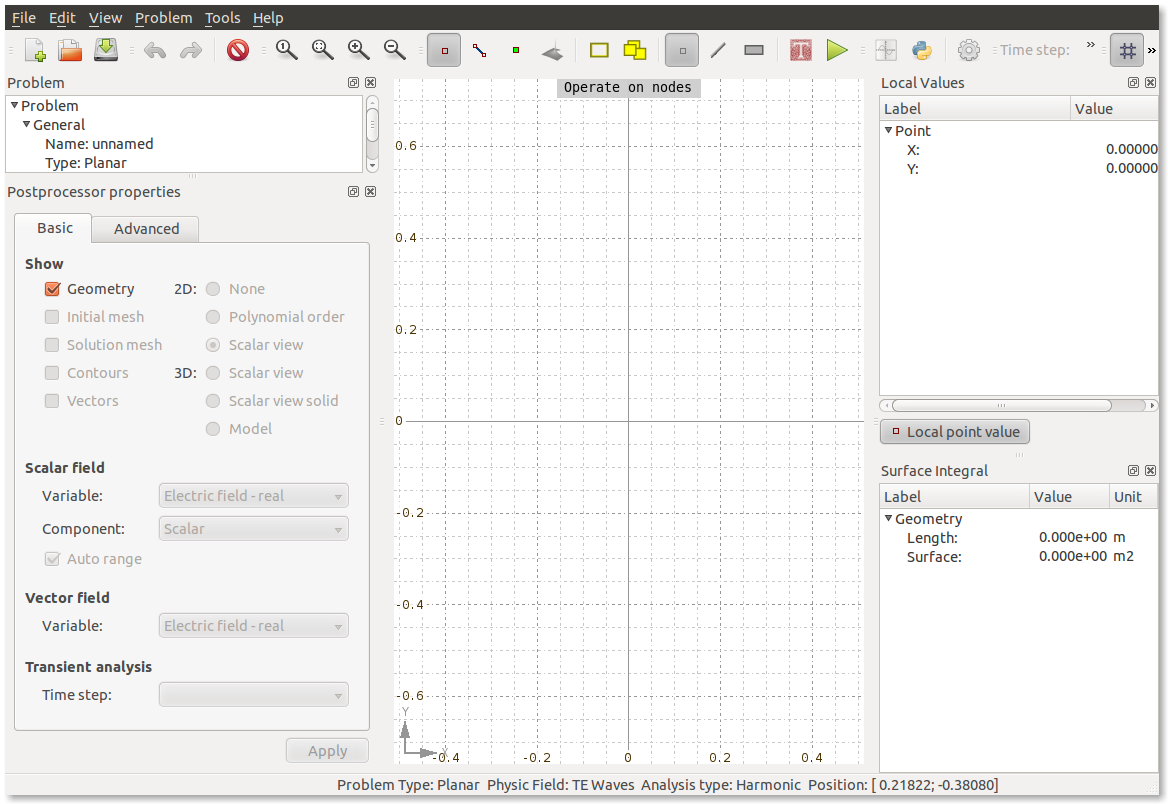
\includegraphics[width=14cm]{sim_agros2d.png}
	\caption{Prostředí programu Agros2D s dialogem pro specifikaci řešeného problému.}
	\label{obr:sim_agros2d}
\end{figure}

Samotný modul pro simulaci elektromagnetického pole tedy využívá z programu Agros2D zmíněný preprocesor pro zadávání dat a postprocesor pro zobrazení výsledků ve 2D a 3D zobrazení. Vlastní numerické řešení zajišťuje knihovna Hermes2D a programový kód je obsažen v modulu  označeném jako TE Waves. V této kapitole jsou popsány výpočetní části, které se týkají především řešení vlnových rovnic, specifikace okrajových podmínek a zadávání materiálových konstant prostředí. 

\section{Předpoklady simulace}
Vzhledem k široké problematice elektromagnetických vln je potřeba pro jejich modelování zavést některé zjednodušení. 
\begin{itemize}
\item {\bf Harmonická analýza} - první předpokladem je řešení vlnové rovnice v harmonickém tvaru (Helmholtzova rovnice)
\begin{displaymath}
	\nabla^{2}\vecfaz E +\faz k^{2}\vecfaz E = 0.
\end{displaymath}
\item {\bf Šíření vln v kartézské souřadnicové soustavě v jediném směru dle osy z} - tento předpoklad platí pro planární problém.
\item {\bf Šíření vln v polární souřadnicové soustavě má pouze tangenciální složku} - uvažujeme pro osově symetrický problém.
\end{itemize}

\section{Metoda konečných prvků}
Základem samotné knihovny Hermes2D je numerické řešení pomocí tzv. metody konečných prvků.
%popis metody, trojúhelníky, ..diskretizace

\section{Řešení harmonické vlnové rovnice knihovnou Hermes2D}
\subsection{Kartézská souřadná soustava} \label{subsec:sim_kar}
Po zavedení zjednodušujících předpokladů vycházíme z rovnice ve tvaru
\begin{equation}
	\nabla^{2}\faz E_{(z)} +\faz k^{2}\faz E_{(z)} = 0
	\label{rce:sim_kar_helmholtz_num} 
\end{equation}
platné na definované oblasti $\Omega$, na které známe okrajové podmínky a ve které chceme dostat výsledné řešení. Tím může být například vnitřní prostor vlnovodu nebo rezonátoru. Pro získání slabé formy k rovnici (\ref{rce:sim_kar_helmholtz_num}) nejprve vyjádříme reálnou a imaginární složku
\begin{displaymath}
	\nabla^{2}(E_R + \mj E_I) + (\omega^{2}\varepsilon\mu - \mj\omega\mu\sigma)(E_R + \mj E_I) = 0,
\end{displaymath}
\begin{displaymath}
	\nabla^{2} E_R + \mj\nabla^{2} E_I + \omega^{2}\varepsilon\mu E_R + \mj\omega^{2}\varepsilon\mu E_I - \mj\omega\mu\sigma E_R + \omega\mu\sigma E_I = 0,
\end{displaymath}
kde reálnou část tvoří
\begin{equation}
	\Re : \nabla^{2} E_R + \omega^{2}\varepsilon\mu E_R + \omega\mu\sigma E_I = 0,
	\label{rce:sim_kar_num_real} 
\end{equation}
a imaginární je vyjádřena
\begin{equation}
	\Im : \nabla^{2} E_I + \omega^{2}\varepsilon\mu E_I - \omega\mu\sigma E_R = 0.
	\label{rce:sim_kar_num_imag} 
\end{equation}
Obě upravené rovnice (\ref{rce:sim_kar_num_real}) a (\ref{rce:sim_kar_num_imag}) je již možné převést do slabých forem, které splňují nulovou Dirichletovu a Neumannovu okrajovou podmínku. Postup převodu spočívá ve vynásobení parciálních diferenciálních rovnic testovací funkcí $v$ a v následné integraci přes oblast řešení $\Omega$ 
\begin{equation}
	\Re : \int_{\Omega}\nabla^{2} E_R\cdot v \dif S + \omega^{2}\varepsilon\mu\int_{\Omega} E_R\cdot v\dif S + \omega\mu\sigma\int_{\Omega} E_I\cdot v\dif S = 0,
	\label{rce:sim_kar_weak_odv_real} 
\end{equation}
\begin{equation}
	\Im : \int_{\Omega}\nabla^{2} E_I\cdot v\dif S + \omega^{2}\varepsilon\mu\int_{\Omega} E_I\cdot v\dif S - \omega\mu\sigma\int_{\Omega} E_R\cdot v\dif S = 0.
	\label{rce:sim_kar_weak_odv_imag} 
\end{equation}
V dalším kroku se aplikuje 1. Greenova identita \cite[příloha A.2]{num} (integrace po částech pro vyšší řády) a tím se konečně získají slabé formy k původním rovnicím (\ref{rce:sim_kar_num_real}) a (\ref{rce:sim_kar_num_imag})
\begin{equation}
	\Re : \int_{\Gamma}\frac{\partial E_R}{\partial n}\cdot v\dif l-\int_{\Omega}\nabla E_R\cdot\nabla v \dif S + \omega^{2}\varepsilon\mu\int_{\Omega} E_R\cdot v\dif S + \omega\mu\sigma\int_{\Omega} E_I\cdot v\dif S = 0,
	\label{rce:sim_kar_weak_real} 
\end{equation}
\begin{equation}
	\Im : \int_{\Gamma}\frac{\partial E_I}{\partial n}\cdot v\dif l-\int_{\Omega}\nabla E_I\cdot\nabla v\dif S + \omega^{2}\varepsilon\mu\int_{\Omega} E_I\cdot v\dif S - \omega\mu\sigma\int_{\Omega} E_R\cdot v\dif S = 0.
	\label{rce:sim_kar_weak_imag} 
\end{equation}
První člen $\int_{\Gamma}\frac{\partial E_R}{\partial n}\cdot v\dif l$ (respektive $\int_{\Gamma}\frac{\partial E_I}{\partial n}\cdot v\dif l$) vyjadřuje Neumanovu okrajovou podmínku. Pokud je podmínka nulová, tak i tyto členy budou nulové. Levé strany rovnic (\ref{rce:sim_kar_weak_real}) a (\ref{rce:sim_kar_weak_imag}) představují bilineární členy daných slabých forem. Lineární členy jsou nulové, neboť se nacházejí na pravých stranách rovnic. 

\subsubsection*{Kód k řešení bilineární části rovnice (\ref{rce:sim_kar_weak_real})}
Pro zápis programového kódu vztahující se k rovnici (\ref{rce:sim_kar_weak_real}) rozdělíme bilineární část na složky reprezentované $E_{R}$ a $E_{I}$. První vyjádříme zápis, který je v programu označen indexem \uv{real\_real}. Rozepsáním operátoru $\nabla$ a numerickým řešením integrálů obdržíme výraz
\begin{equation}
	-\sum_{i=0}^{n}\mathrm{w}_{t}[i]\bigg(\frac{\partial E_R}{\partial x}\cdot \frac{\partial v}{\partial x} + \frac{\partial E_R}{\partial y}\cdot \frac{\partial v}{\partial y} \bigg) + \omega^{2}\varepsilon\mu\sum_{i=0}^{n}\mathrm{w}_{t}[i]\bigg(E_R\cdot v\bigg),
	\label{rce:sim_kar_weak_real_real_num} 
\end{equation}
Vlastní programový kód, který implemetuje bilineární část (\ref{rce:sim_kar_weak_real_real_num}), je následující

\begin{verbatim}
template<typename Real, typename Scalar>
Scalar rf_matrix_form_real_real(int n, double *wt, Func<Real> *u_ext[], Func<Real> *u,
                                    Func<Real> *v, Geom<Real> *e, ExtData<Scalar> *ext)
{
   return - int_grad_u_grad_v<Real, Scalar>(n, wt, u, v)
   + sqr(2 * M_PI * frequency) * (rfLabel[e->elem_marker].permeability * MU0)
   * (rfLabel[e->elem_marker].permittivity * EPS0) * int_u_v<Real, Scalar>(n, wt, u, v);
}
\end{verbatim}
Obdobným způsobem postupujeme u druhé složky bilineární části vyjádřené pomocí $E_I$. Index funkce v programu se změní na \uv{real\_imag}
\begin{equation}
 \omega\mu\sigma\sum_{i=0}^{n}\mathrm{w}_{t}[i]\bigg(E_I\cdot v\bigg)
	\label{rce:sim_kar_weak_real_imag_num} 
\end{equation}
Vztah \ref{rce:sim_kar_weak_real_imag_num} se analogicky zapíše jako
\begin{verbatim}
template<typename Real, typename Scalar>
Scalar rf_matrix_form_real_imag(int n, double *wt, Func<Real> *u_ext[], Func<Real> *u,
                                     Func<Real> *v, Geom<Real> *e, ExtData<Scalar> *ext)
{
   return + 2 * M_PI * frequency * (rfLabel[e->elem_marker].permeability * MU0) 
   * rfLabel[e->elem_marker].conductivity * int_u_v<Real, Scalar>(n, wt, u, v);
}
\end{verbatim}

\subsubsection*{Kód k řešení bilineární části rovnice (\ref{rce:sim_kar_weak_imag})}
Postup je naprosto totožný jako u slabé formy reálné složky výchozí rovnice. Tudíž opět rozdělíme bilineární část na 2 části dle $E_R$ a $E_I$. Dále zavedeme numerickou integraci a zapíšeme vzniklé výrazy do programového kódu. Pro index \uv{imag\_real} platí
\begin{equation}
 -\omega\mu\sigma\sum_{i=0}^{n}\mathrm{w}_{t}[i]\bigg(E_I\cdot v\bigg)
	\label{rce:sim_kar_weak_imag_real_num} 
\end{equation}
\begin{verbatim}
template<typename Real, typename Scalar>
Scalar rf_matrix_form_imag_real(int n, double *wt, Func<Real> *u_ext[], Func<Real> *u,
									Func<Real> *v, Geom<Real> *e, ExtData<Scalar> *ext)
{
    return - 2 * M_PI * frequency * (rfLabel[e->elem_marker].permeability * MU0) 
    * rfLabel[e->elem_marker].conductivity * int_u_v<Real, Scalar>(n, wt, u, v);
}
\end{verbatim}
Nakonec pro označení \uv{imag\_imag}
\begin{equation}
	-\sum_{i=0}^{n}\mathrm{w}_{t}[i]\bigg(\frac{\partial E_I}{\partial x}\cdot \frac{\partial v}{\partial x} + \frac{\partial E_I}{\partial y}\cdot \frac{\partial v}{\partial y} \bigg) + \omega^{2}\varepsilon\mu\sum_{i=0}^{n}\mathrm{w}_{t}[i]\bigg(E_I\cdot v\bigg),
	\label{rce:sim_kar_weak_imag_imag_num} 
\end{equation}
\begin{verbatim}
template<typename Real, typename Scalar>
Scalar rf_matrix_form_imag_imag(int n, double *wt, Func<Real> *u_ext[], Func<Real> *u,
                                    Func<Real> *v, Geom<Real> *e, ExtData<Scalar> *ext)
{
    return - int_grad_u_grad_v<Real, Scalar>(n, wt, u, v) 
    + sqr(2 * M_PI * frequency) * (rfLabel[e->elem_marker].permeability * MU0) 
    * (rfLabel[e->elem_marker].permittivity * EPS0) * int_u_v<Real, Scalar>(n, wt, u, v);
}
\end{verbatim}

\subsubsection*{Zápis lineárních členů rovnic (\ref{rce:sim_kar_weak_real}) a (\ref{rce:sim_kar_weak_imag}).}
Lineární členy jsou vyjádřeny jako pravé strany rovnic (\ref{rce:sim_kar_weak_real}) a (\ref{rce:sim_kar_weak_imag}). Jsou tudíž nulové, ale pro vlastní numerické řešení je potřeba tuto informaci doplnit do programového kódu. Vzhledem k tomu, že řešená rovnice je komplexního charakteru je potřeba doplnit tyto dvě funkce 

\begin{verbatim}
template<typename Real, typename Scalar>
Scalar rf_vector_form_real(int n, double *wt, Func<Real> *u_ext[], Func<Real> *v,
                                               Geom<Real> *e, ExtData<Scalar> *ext)
{
    return 0.0;
}
\end{verbatim}
\begin{verbatim}
template<typename Real, typename Scalar>
Scalar rf_vector_form_imag(int n, double *wt, Func<Real> *u_ext[], Func<Real> *v, 
                                              Geom<Real> *e, ExtData<Scalar> *ext)
{
    return 0.0;
}
\end{verbatim}
Zmíněné funkce pro řešení Helmholtzovy rovnice (\ref{rce:sim_kar_helmholtz_num}) je dále potřeba zaregistrovat ve třídě \textsc{WeakForm} následujícím způsobem
\begin{verbatim}
  wf->add_matrix_form(0, 0, callback(rf_matrix_form_real_real));
  wf->add_matrix_form(0, 1, callback(rf_matrix_form_real_imag));
  wf->add_matrix_form(1, 0, callback(rf_matrix_form_imag_real));
  wf->add_matrix_form(1, 1, callback(rf_matrix_form_imag_imag));
  wf->add_vector_form(0, callback(rf_vector_form_real))
  wf->add_vector_form(1, callback(rf_vector_form_imag));
\end{verbatim}

\subsection{Polární souřadná soustava}
Řešení vlnové rovnice v polárních souřadnicích vychází z rovnice
\begin{equation}
	\nabla\times(\nabla\times\vecfaz E) +\faz k^{2}\vecfaz E = 0.
	\label{rce:sim_pol_helmholtz_num} 
\end{equation}
Po zavedení zjednodušení, že výsledné řešení má pouze tangenciální složku, můžeme rovnici \ref{rce:sim_pol_helmholtz_num} snadno upravit. Nejprve vyjádříme vnitřní rotaci
\begin{displaymath}
	\nabla\times \frac{1}{r}\Bigg|
	\begin{array}{ccc}
\hat{r} & r\hat{\alpha} & \hat{z} \\
\frac{\partial}{\partial r} & \frac{\partial}{\partial \alpha} & \frac{\partial}{\partial z} \\
0 & r\faz E_{\alpha} & 0\\
\end{array}\Bigg| +\faz k^{2}\faz E_{\alpha} = 0,
\end{displaymath}
\begin{equation}
\nabla\times \Bigg[\hat{r}\bigg(-\frac{1}{r}\cdot\frac{\partial r\faz E_{\alpha}}{\partial z}\bigg) + \hat{\alpha}\bigg(0\bigg) + \hat{z}\bigg(\frac{1}{r}\cdot\frac{\partial r\faz E_{\alpha}}{\partial r}\bigg) \Bigg]+\faz k^{2}\faz E_{\alpha} = 0.
	\label{rce:sim_pol_rotace1}
\end{equation}
Analogickým způsobem upravíme vnější rotaci ve vztahu (\ref{rce:sim_pol_rotace1})
\begin{displaymath}
	\frac{1}{r}\Bigg|
	\begin{array}{ccc}
\hat{r} & r\hat{\alpha} & \hat{z} \\
\frac{\partial}{\partial r} & \frac{\partial}{\partial \alpha} & \frac{\partial}{\partial z} \\
-\frac{1}{r}\cdot\frac{\partial r\faz E_{\alpha}}{\partial z} & 0 & \frac{1}{r}\cdot\frac{\partial r\faz E_{\alpha}}{\partial r}\\
\end{array}\Bigg| +\faz k^{2}\faz E_{\alpha} = 0,
\end{displaymath}
\begin{equation}
\Bigg[\hat{r}\bigg(\frac{1}{r}\cdot\frac{\partial}{\partial \alpha}\cdot\frac{1}{r}\frac{\partial r\faz E_{\alpha}}{\partial r}\bigg) + \hat{\alpha}\bigg(-\frac{\partial}{\partial z}\cdot\frac{1}{r}\cdot\frac{\partial r\faz E_{\alpha}}{\partial z} - \frac{\partial}{\partial r}\cdot\frac{1}{r}\cdot\frac{\partial r\faz E_{\alpha}}{\partial r}\bigg) + \hat{z}\bigg(\frac{1}{r}\cdot\frac{\partial}{\partial \alpha}\cdot\frac{1}{r}\frac{\partial r E_{\alpha}}{\partial z}\bigg) \Bigg]+\faz k^{2}\faz E_{\alpha} = 0.
	\label{rce:sim_pol_rotace2}
\end{equation}
Ve výsledném vztahu (\ref{rce:sim_pol_rotace2}) zanedbáme všechny ostatní složky kromě té, která respektuje souřadnici $\hat{\alpha}$. Dostaneme rovnici
\begin{displaymath}
-\frac{\partial}{\partial z}\cdot\frac{1}{r}\cdot\frac{\partial r\faz E_{\alpha}}{\partial z} - \frac{\partial}{\partial r}\cdot\frac{1}{r}\cdot\frac{\partial r\faz E_{\alpha}}{\partial r}+\faz k^{2}\faz E_{\alpha} = 0,
\end{displaymath}
kterou upravíme do podoby
\begin{equation}
-\frac{\partial^{2}E_{\alpha}}{\partial z^{2}}-\frac{\partial^{2}E_{\alpha}}{\partial r^{2}}-\frac{1}{r}\cdot\frac{\partial E_{\alpha}}{\partial r} + \frac{E_{\alpha}}{r^{2}} +\faz k^{2}\faz E_{\alpha} = 0.
	\label{rce:sim_pol_helmholtz_upravena}
\end{equation}
Tento vztah představuje vyjádření Helmholtzovy rovnice v polárních souřadnicích, při uvažování výše uvedených předpokladů simulace. Pro zápis programového kódu k vyřešení rozložení pole při osové symetrii je potřeba, stejným způsobem jako v podkapitole \ref{subsec:sim_kar}, odvodit slabou formu k rovnici (\ref{rce:sim_pol_helmholtz_upravena}) 
splňující Dirichletovu i Neumannovu okrajovou podmínku. 

\subsubsection*{Numerické řešení rovnice (\ref{rce:sim_pol_helmholtz_upravena})}
Bilineární člen dané slabé formy s indexem \uv{real\_real} lze po zavedení numerické integrace zapsat jako
\begin{displaymath}
-\sum_{i=0}^{n}\mathrm{w}_{t}[i]\bigg(\frac{\partial E_{\alpha R}}{\partial z}\cdot \frac{\partial v}{\partial z} + \frac{\partial E_{\alpha R}}{\partial r}\cdot \frac{\partial v}{\partial r} \bigg) - \frac{1}{r}\sum_{i=0}^{n}\mathrm{w}_{t}[i]\bigg(\frac{\partial E_{\alpha R}}{\partial r}\cdot v\bigg) +
\end{displaymath}
\begin{equation}
	 + \frac{1}{r^{2}}\sum_{i=0}^{n}\mathrm{w}_{t}[i]\bigg(E_{\alpha R}\cdot v\bigg) + \omega^{2}\varepsilon\mu\sum_{i=0}^{n}\mathrm{w}_{t}[i]\bigg(E_{\alpha R}\cdot v\bigg).
	\label{rce:sim_pol_bilinear_real_real} 
\end{equation}
Je zřejmé, že forma označená \uv{real\_imag} vyjde identicky jako v případě kartézské souřadné soustavy, neboť člen $+\faz k^{2}\faz E_{\alpha}$ v rovnici (\ref{rce:sim_pol_helmholtz_upravena}) je formálně stejný se vztahem (\ref{rce:sim_kar_helmholtz_num}). Platí tedy
\begin{equation}
 \omega\mu\sigma\sum_{i=0}^{n}\mathrm{w}_{t}[i]\bigg(E_{\alpha I}\cdot v\bigg).
	\label{rce:sim_pol_bilinear_real_imag} 
\end{equation}
Slabým formám vycházející z imaginární části z původní rovnice (\ref{rce:sim_pol_helmholtz_upravena}) odpovídá vyjádření
\begin{equation}
 -\omega\mu\sigma\sum_{i=0}^{n}\mathrm{w}_{t}[i]\bigg(E_{\alpha R}\cdot v\bigg)
	\label{rce:sim_pol_bilinear_imag_imag} 
\end{equation}
pro \uv{imag\_real}, což je opět ze stejného důvodu identické s kartézskou souřadnou soustvou. Nakonec indexu \uv{imag\_imag} odpovídá
\begin{displaymath}
-\sum_{i=0}^{n}\mathrm{w}_{t}[i]\bigg(\frac{\partial E_{\alpha I}}{\partial z}\cdot \frac{\partial v}{\partial z} + \frac{\partial E_{\alpha I}}{\partial r}\cdot \frac{\partial v}{\partial r} \bigg) - \frac{1}{r}\sum_{i=0}^{n}\mathrm{w}_{t}[i]\bigg(\frac{\partial E_{\alpha I}}{\partial r}\cdot v\bigg) +
\end{displaymath}
\begin{equation}
	 + \frac{1}{r^{2}}\sum_{i=0}^{n}\mathrm{w}_{t}[i]\bigg(E_{\alpha I}\cdot v\bigg) + \omega^{2}\varepsilon\mu\sum_{i=0}^{n}\mathrm{w}_{t}[i]\bigg(E_{\alpha I}\cdot v\bigg).
	\label{rce:sim_pol_bilinear_real_real} 
\end{equation}
Vzhledem k nulové pravé straně řešené výchozí rovnice (\ref{rce:sim_pol_helmholtz_upravena}) bude lineární člen  v tomto případě opět nulový.

\subsection{Numerická integrace}

\section{Okrajové podmínky}
Pro řešení diferenciálních rovnic popisující chování elektromagnetického pole v dané oblasti $\Omega$ je třeba znát okrajové podmínky na hranicích. Účelem je specifikovat chování výsledné funkce, případně derivace této funkce, v daných bodech ležících na okraji řešené oblasti. Při popisu fyzikálních polí pomocí diferenciálních rovnic se užívá Dirichletova, Neumannova nebo Newtonova (smíšená) okrajová podmínka.
\begin{itemize}
\item {\bf Dirichletova okrajová podmínka} - předepisuje na hranici $\Gamma$ hodnotu funkce $E_{(z)}$, která může být obecně závislá na čase nebo na souřadnicích
\begin{displaymath}
	E_{(z)}|_{\Gamma} = f_{Dir}(x,y,z,t). 
\end{displaymath}
\item {\bf Neumannova okrajová podmínka} - na okraji řešené oblasti definuje tato podmínka definuje hodnotu normálové derivace funkce $\frac{\partial E_{(z)}}{\partial n}$
\begin{displaymath}
	\frac{\partial E_{(z)}}{\partial n}|_{\Gamma} = f_{Neu}(x,y,z,t). 
\end{displaymath}
\item {\bf Newtonova okrajová podmínka} - neboli smíšená kombinuje obě předchozí uvedené okrajové podmínky. Na hranici $\Gamma$ tak specifikuje kombinaci hodnoty funkce $E_{(z)}$ a její normálové derivace $\frac{\partial E_{(z)}}{\partial n}$
\begin{displaymath}
	\bigg(\frac{\partial E_{(z)}}{\partial n} + E_{(z)}\bigg)|_{\Gamma} = f_{New}(x,y,z,t). 
\end{displaymath}
\end{itemize}

\subsection{Okrajové podmínky v simulačním modulu}
Při řešení problémů vztahující se k elektromagnetickému poli je možné použít na řešenou oblast několik typů okrajových podmínek, které se zadávají v dialogu \uv{new boundary condition}. Ten je možné zpřístupnit po pravém kliknutí na pracovní plochu a vybrání daného odkazu, případně je možné se na něj dostat klávesovou zkratkou Alt + B. Po zadání označení se vybere v rozbalovacím menu některá z definovaných okrajových podmínek.

\subsubsection*{Electric field}
První možností je zadat Dirichletovu podmínka na určité hranici $\Gamma$. Hodnotu okrajové podmínky zadáme jako komplexní číslo ve formátu reálné a imaginární složky, jak je znázorněno na obrázku \ref{obr:sim_BC_electric_field} pro číslo $0 + \mj 0$.
\begin{figure}[!h]
	\centering
	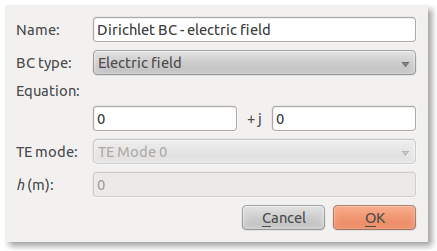
\includegraphics[width=7cm]{sim_BC_electric_field.png}
	\caption{Zadání Dirichletovy podmínky $0 + \mj 0$ pro elektrickou složku pole.}
	\label{obr:sim_BC_electric_field}
\end{figure}

\subsubsection*{Magnetic field}
\subsubsection*{Matched boundary}
\subsubsection*{Port}

\section{Vlastnosti prostředí}


\section{Postup řešení úloh v aplikaci Agros2D}

\section{Zobrazení výsledků řešení}


